\documentclass[tikz,border=2pt]{standalone}
\usepackage{amsmath,amssymb}
\usetikzlibrary{arrows.meta}
\begin{document}
% Induction as dominoes: the base case pushes P(0) (green), the inductive step P(k) => P(k+1)
% links every domino to the next (blue arcs), so P(n) holds for every natural number n (green line).
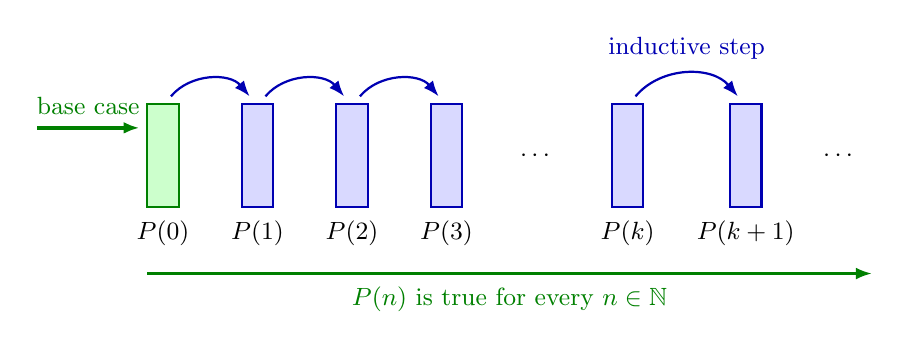
\begin{tikzpicture}[font=\small, >={Latex[length=2mm]}]
  % dominoes: x position / label
  \foreach \x/\l in {0/0, 1.2/1, 2.4/2, 3.6/3, 5.9/k, 7.4/k+1} {
    \filldraw[thick, draw=blue!70!black, fill=blue!15] (\x-0.2,0) rectangle (\x+0.2,1.3);
    \node[below] at (\x,-0.05) {$P(\l)$};
  }
  % the first domino is the base case
  \filldraw[thick, draw=green!50!black, fill=green!20] (-0.2,0) rectangle (0.2,1.3);
  \node at (4.75,0.65) {$\cdots$};
  \node at (8.6,0.65) {$\cdots$};
  % base case: push the first domino
  \draw[->, very thick, green!50!black] (-1.6,1.0) -- (-0.3,1.0);
  \node[green!50!black, above] at (-0.95,1.05) {base case};
  % inductive step: each domino knocks over the next
  \foreach \a/\b in {0/1.2, 1.2/2.4, 2.4/3.6, 5.9/7.4} {
    \draw[->, thick, blue!70!black] (\a+0.1,1.4) to[bend left=50] (\b-0.1,1.4);
  }
  \node[blue!70!black, above] at (6.65,1.75) {inductive step};
  % conclusion
  \draw[->, thick, green!50!black] (-0.2,-0.85) -- (9.0,-0.85);
  \node[green!50!black, below] at (4.4,-0.9) {$P(n)$ is true for every $n\in\mathbb{N}$};
\end{tikzpicture}
\end{document}
